% -----------------------------------------------
% Template for JIM
%     jim.sty -> style file
% By Eloi Batlle (eloi@iua.upf.es), changes for 
% ICMC by Bram de Jong (bdejong@iua.upf.es)
% changes for JIM 2007 by Dominique Fober (fober@grame.fr)
% changes for JIM 2009 by Olivier Tache (olivier.tache@imag.fr)
% -----------------------------------------------

\documentclass{article}
\usepackage{jim,amsmath}
\usepackage[utf8]{inputenc}
\usepackage[francais]{babel}
\usepackage[T1]{fontenc}
\usepackage{enumitem}
\usepackage{graphicx}
\usepackage{balance}
\usepackage{ifpdf}
\usepackage{hyperref}
\usepackage{amssymb,amsmath} 
\usepackage{verbatim}
\usepackage{color}

\definecolor{mygrey}{gray}{0.93}

\newcommand{\OSC}[1]	{{\fontsize{10pt}{10pt} \selectfont\texttt{#1}}}
\newcommand{\oper}[1]	{\textcolor{figRed}{#1}}
\newcommand{\param}[1]	{\textcolor{figOrange}{#1}}
\newcommand{\prefix}[1]	{\textcolor{figBlue}{#1}}

\newcommand{\note}[1]{\textcolor{red}{(#1)}}

\newcommand{\lowTilde}{\texttildelow}
\newcommand{\tab}{\hspace*{4mm}}
\let\olditemize\itemize
\let\oldenditemize\enditemize
\renewenvironment{itemize} 	{\olditemize \renewcommand{\labelitemi}{$\bullet$} \setlength{\itemsep}{0mm}}{\oldenditemize}

\newcommand{\sample}[1]		{\vspace{-0.2em}\begin{center}\colorbox{mygrey}{\begin{minipage}[t]{0.97\columnwidth} {\small \texttt{#1}}\end{minipage}}\end{center}}


% Title.
% ------
\title{Un model événementiel du temps pour INScore.}

% Single \textsc{address}
% To use with only one author or several with the same address
% ---------------
\oneauthor
  {D. Fober} {Grame \\
  Centre nationale de création musicale \\
  Lyon - France \\
     {\tt {\small \{fober\}@grame.fr}}}

% Two addresses
% --------------
%\twoauthors
%  {First author} {School \\ Department}
%  {Second author} {Company \\ Address}

% Three addresses
% --------------
%\threeauthors
%  {Auteur 1} {Organisme \\ Adresse électronique}
%  {Auteur 2} {Organisme \\ Adresse électronique}
%  {Auteur 3} {Organisme \\ Adresse électronique}

\begin{document}
%
\maketitle
%
\begin{abstract}
INScore est un environnement pour la conception de partition interactives augmentées, tourné vers des usages non conventionnels de la notation musicale. Dans cet environnement, bien que tous les objets de la partition aient une dimension temporelle, le temps reste statique i.e. que la date (ou la durée) d'un objet ne change pas, sauf à réception d'un message qui ne peut être produit que de manière externe ou événementielle. INScore n'inclut donc pas de gestionnaire du temps au sens classique du terme. 
Ce choix de conception a été dicté par le fait que le système est conçu pour des usages couplés avec des logiciels en charge de l'environnement sonore, qui ont des contraintes de temps-réel plus strictes que l'environnement graphique d'INScore.
Toutefois, la nécessité d'introduire un gestionnaire du temps \emph{dynamique} a progressivement émergé, conduisant à un modèle original du temps, à la fois \emph{événementiel} et continu. C'est ce modèle qui est présenté et ses propriétés dans l'environnement d'INScore.
\end{abstract}

%==============================================================
\section{Introduction}\label{sec:introduction}

Ici on détaille pourquoi le temps est resté statique jusqu'à présent et pourquoi on l'introduit maintenant.
On fait également un survol des représentations du temps dans différents environnements : OM, AnteScofo, iScore, les tuiles de David, Max, etc. et on décrit l'originalité du modèle proposé.


%==============================================================
\section{Le modèle du temps}\label{overview}

Le modèle du temps proposé est à la fois événementiel et continu : le temps est vu comme un intervalle fini, borné par des événements. Le temps est \emph{activé} par un événement pour une durée donnée et produit un événement à la fin de cette durée. La durée d'activation est exprimée en temps absolu. Nous parlerons de \emph{segment temporel} pour désigner la durée d'activation du temps, d'événement \emph{entrant} pour désigner l'événement déclencheur d'un segment temporel, et d'événement \emph{sortant} pour l'événement produit à la fin de ce segment.

Chaque objet du modèle INScore possède ces propriétés \emph{d'activation} temporelle et peut donc gérer une logique du temps indépendante. Un exemple d'activation du temps pour 3 objets d'une partition est illustré en figure \ref{fig:temps}.
  
\begin{figure}[h]
   \centering
   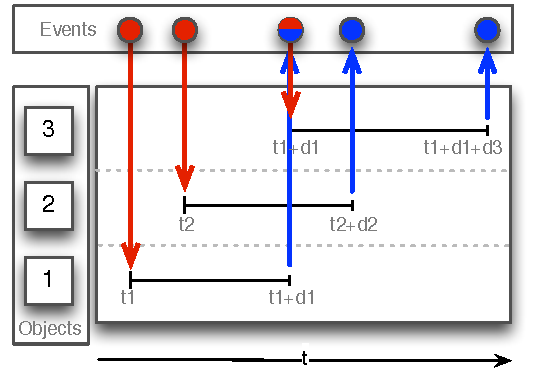
\includegraphics[width=0.95\columnwidth]{imgs/temps}
   \caption{Une vue du temps pour 3 objets distincts. Les événements en rouge activent des segments temporels, ceux en bleu sont produits à l'échéance de ces segments. A noter que l'événement en sortie de l'objet 1 est également l'événement en entrée de l'objet 3.}
   \label{fig:temps}
\end{figure}

Pour INScore, le temps n'est visible qu'à travers les propriétés graphiques des objets de la partitions. L'unique manière de visualiser les relations temporelles entre les objets consiste à les synchroniser : on parle alors de \emph{synchronisation temporelle dans l'espace graphique} \cite{fober:10b}, mais le temps reste \emph{statique} (au sens évoqué précédement). 

Comme le rappelle Giavitto \cite{giavitto:hal-00960989}, temps physique et temps perçu ne sont pas réductibles et pour mesurer le passage du temps \emph{de manière analogue à la vitesse d'un fleuve, il faudrait mesurer combien l'état temporel des choses a passé au bout d'un temps donné}, pour convenir finalement \emph{qu'il s'écoule une minute par minute}. Afin de rendre compte de cette vitesse, nous proposons un renversement de perspective qui consiste à mesurer l'écoulement du temps à travers ses effets visibles : à chaque fonction du temps est associée une valeur et c'est l'évolution de cette valeur qui va rendre compte de l'évolution du temps. Pour INScore, cette valeur pourra être associée à un attribut graphique arbitraire d'un objet, ce qui permet ainsi d'introduire les effets du temps dans l'espace graphique.


%==============================================================
\section{Définitions}
%--------------------------------------------------------
\subsection{Séquence temporelle}
Nous définissons une \emph{séquence temporelle} comme un triplet
%\begin{equation}
%\[\mathbb{S} = ( e_i, d, f, e_j )\]
\[\mathbb{S} = ( e_i, d, e_j )\]
%\end{equation}
où :
\begin{itemize}
	\item $e_i$ et $e_j$ sont respectivement les événements entrants et sortants 
	\item $d$ est la durée du segment temporel
%	\item $f$ est une fonction du temps définie sur $[0, d]$
\end{itemize}
L'activation d'une séquence temporelle $\mathbb{S}$ peut-être vue comme une fonction qui prend un événement en entrée et produit une événement un sortie.
Pour désigner une séquence activée à la date $t$, nous noterons : 
\begin{equation}
\mathbb{S}(t, e_i) \rightarrow (t + d, e_j)
\label{eq1}
\end{equation}
%Enfin $t(e)$ fait référence à la date d'un événement $e$. Pour la séquence désignée en (\ref{eq1}), $t(e_j) = t(e_i) + d$

%--------------------------------------------------------
\subsection{Instantiation}
Une séquence temporelle est toujours instantiée dans le contexte d'un objet de la partition. Nous désignerons par $\mathbb{S}_t(O_n)$, la séquence temporelle associée à un objet $O_n$, produite par un événement entrant à la date $t$.\\





%==============================================================
\section{Propriétés}



%==============================================================
\section{Conclusions}


%\balance
\bibliographystyle{ieeetr}
\bibliography{../interlude}

\end{document}
